To the best of our knowledge, Golden Gate, originally MIDAS II, is the first
open-source, optimizing FAME compiler. The content chapter follows that
contained in our 2019 ICCAD publication~\cite{GoldenGate}, but better
contextualizes the design of the compiler against MIDAS and elaborates on
implementation details pertinent to the later chapters of this dissertation.
For a second perspective, we direct the interested reader to Albert Magyar's
dissertaion. Code references in this chapter will refer to sources in FireSim version 1.8.0~\footnote{https://github.com/firesim/firesim/tree/1.8.0}.

\section{Design Objectives}

We had the following objectives when we set to design Golden Gate:

\begin{enumerate}
\item \textbf{Maintain FireSim feature-completeness.} We wanted the ability to
drop in Golden Gate as a replacement for MIDAS in a future release, with the
only immediate user-facing difference being the availability of new
optimizations.  As a side effect of a more sophisticated compiler, we expected
compile times would increase, however, we wanted unoptimized simulators to have
approximately the same simulation perfomance and resource utilization as those generated by MIDAS.

\item \textbf{Minimize user modification to the ASIC RTL.} It is all too easy to
provide a crutch the compiler by requiring the user make RTL changes to expose optimization opportunities. The difficulty is these changes can be
invasive: in the best case, behavior-preseving modifications to the design's
module hierachy, in worst, functional RTL changes. These changes can introduce
performance descrepancies between the ASIC and emulation-variants of the
design, and may come at the expense of ASIC QoR. While we fully expect that
there will be times where these changes are desired, we made no such
changes in the Rocket-Chip or BOOM code bases to implement the optimizations
desribed in our ICCAD paper.

%\item \textbf{Make it possible to optimize blocks that are combinationally coupled in the target.}
%If we want to avoid relying the user to expose optimization opportunities in their ASIC source,
%our compiler needs to be more flexible in identifying optimization candidates.

\item \textbf{Provide a mechanism to rigorously verify the simulator.} Many of
the RAMP-style optimizations introduce considerable complexity into the
simulator, making the resulting system harder to debug, and reason about
effectively. A buggy optimization can introduce simulation deadlock, or false
bugs in the target design that would not appear otherwise. More insidiously,
the optimization may produce functionally correct simulator, with slightly
different timing behavior, introducing difficult-to-detect performance
descrepancies. We wanted users to trust the compiler wasn't changing their
design beneath their feet.

\item \textbf{Enable the use of FireSim as a library for hardware emulation.}
MIDAS and FireSim had developed in isolation of the chip-design projects
ongoing at UCB-BAR, and used custom forks of many of the same hardware and
target-software libraries. This made it challenging for chip designers to run
their designs in FireSim without extensive help from a FireSim developer to make their design "FireSim-compatible". We
wanted to make it possible to include FireSim in a chip-like project --- this
would become Chipyard~\cite{Chipyard} --- to support seemlessly pushing chip
designs through an emulation flow.
\end{enumerate}

Our desire to maintain FireSim feature-completeness made it clear from the
outset that a complete redesign of the compiler was untenable in a reasonable timeframe. Instead, Golden
Gate was developed as a series of incremental reimplementations key phases of
MIDAS. This let us continually build functional emulators of the same designs
supported in mainline FireSim. We began by intoducing support for
optimizations, while maintaining the existing endpoint support and compiler
interface~(Sections~\ref{sec:midas-endpoints} and \ref{sec:midas-chisel-api}
respectively).

To enable optimizations, we considered a few possibilities such as leaning on
the endpoint system and user modifications to the target RTL (this violates
objective 2), or using specialized transformations to implement optimizations
directly as modifications to the hub model~(this made it more difficult to
achieve object 3).

Ultimately, what we settled on was a compiler organization that leverages the
LI-BDN target formalism and extensive module-hierarchy modifications to coerce
the target into a form such that the top-level modules of the design map
bijectively into units in the resulting simulator graph. LI-BDN removes the
explicit need for channels and permits modules (and thus resulting units) to be
combinationally coupled, widening the scope of potential optimizations. We
acknowledge that forcing optimizations to apply only at registered boundaries
between units -- a requirement of a channel-bootstrapped formalism -- would
produce simulators with better FMR, this would add complexity to passes in the
compiler and might make some optimizations infeasible.  We also note that these
sorts of optimizations not fundamentally precluded by LI-BDN: when an edge
between two LPs is driven by an output port with no combinational dependency on
an input, it may be possible to implement that edge using flow queue to save a
cycle of transmission latency.

Moving to an LI-BDN formalism resolves a number of other modeling
challenges MIDAS users face.  Requiring that non-wire-channels be injected
between endpoints and the hub unit was too restrictive in some cases where
the user wishes to model a combinational path that propagates through an
endpoint. Another challenge was defining the reset semantics of these
stateful channels.  MIDAS relies on FPGA programming to properly initialize
these channels, however they are not held in target reset  during
simulation: it is purely coincidental that the hub model does not
spuriously enqueue target data into queue-type channels while parts of the
hub are under target reset. For a time, MIDAS would broadcast target reset
tokens to channels and endpoints, but too is fraught as resets driving
registers in the hub maybe different from this special-cased global reset.
Instead of requiring that user specify this reset for each channel, LI-BDN
can sidestep these issues entire by removing the need for stateful
channels, allowing the compiler to assume fewer things about target.

The second phase of Golden Gate's development addressed the fourth objective,
and required a redesign of the compiler interface and endpoint system. Here, we
decouple Golden Gate from the target-elaboration: the compiler accepts a FIRRTL
file and annotations which describes a closed target system. \emph{Bridges}
replace endpoints and are instantiated throughout the target module hierarchy
during target elaboration. The compiler no longer matches on the Chisel IO of
the top-level module, instead \emph{BridgeAnnotations} tied to these modules
provide the class name of the chisel generator Golden Gate should invoke.

\section{Holdovers From MIDAS}
%What hasn't changed:
%- Integration into FireSim largely unchanged
%- Still FPGA-CPU cohosted
%- Still same primary three resources
%- Simulation flow the same; Driver unchanged
%
%- Reference the version of Golden Gate we're using. After the GG paper.

\section{Compiler Input \& Target Specification}

Golden Gate, unlike MIDAS, accepts a "closed" description of the target
consisting of FIRRTL and annotations. We show a pictoral example of this with
typical Chipyard-generated SoC in Figure~\ref{fig:gg-target}. By closed, in
this case we mean that the
top-level module has no I/O -- the user instantiates their chip in a top-level
environment or harness module and drives the chip-interfaces using target-RTL
or, if that is insufficient, bridges. Bridges are so named because they span
the host and target domains -- the \emph{target-side} of a bridge consists of a
Chisel module, generally a black box, whose instance is annotated with a BridgeAnnotation,
and whose ports are annotated with channel annotations that specify how the
interface should divided into token streams. The \emph{host-side} is a unit (a
primitive LI-BDN) that implements that black-box module, and just like
endpoints, these units consist of a module (\emph{BridgeModule} and a driver
(\emph{BridgeDriver}). In addition to Bridge-related annotations, users
identify specific structures for optimization by annotating them. As in MIDAS, additional compiler-side features are controlled using a
parameters instance, again to enable instrumentation passes as they would in
MIDAS. Additional host and target FIRRTL tranforms are provided in this
parameters instance.

\begin{figure}
    \centering
    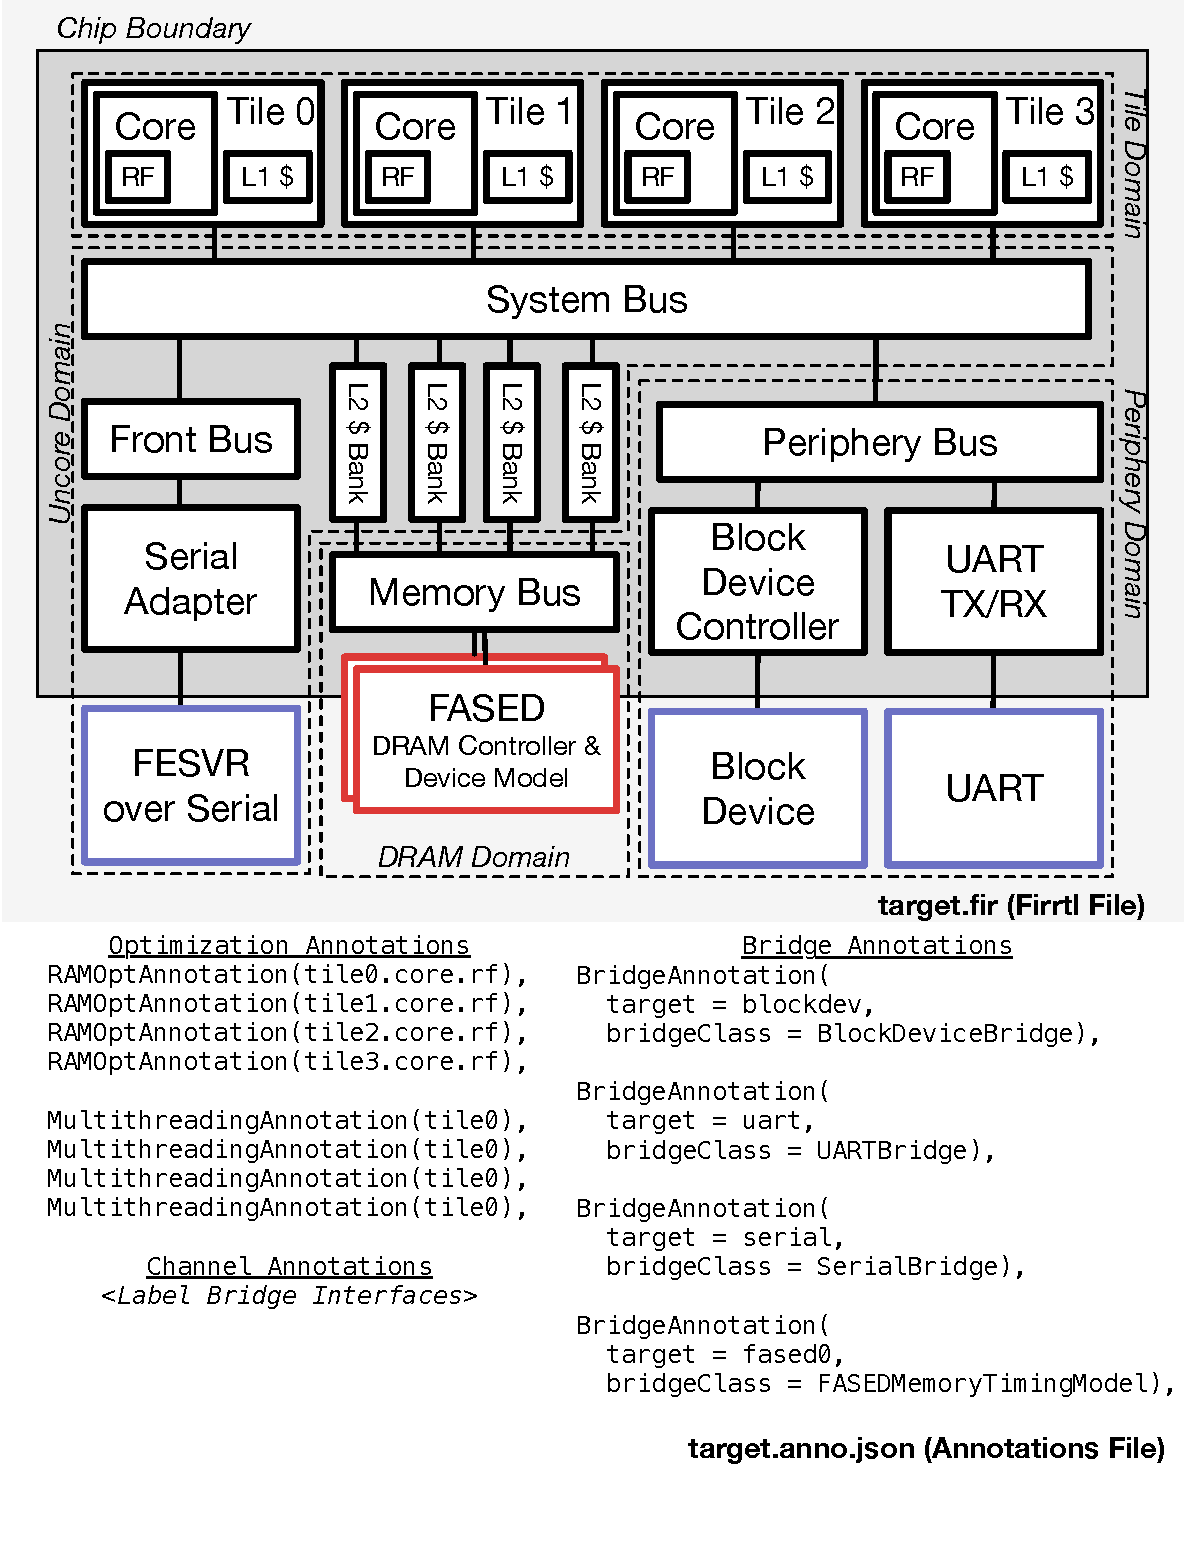
\includegraphics[width=0.99\textwidth]{figures/gg-target.pdf}
    % graffle2pdf -c gg-target midas-graphics/graffle/midas2-target.graffle figures/gg-target.pdf
    \caption{A pictoral representation of a typical input to Golden Gate.}
    \label{fig:gg-target}
\end{figure}

Since it does not require access to unserializable Scala
types like MIDAS, Golden Gate can be invoked as standalone application on an
elaborated target. This permits running the
compiler on a target elaborated in a different context, that may use a
different version of Chisel, FIRRTL, and Rocket Chip than those the compiler
itself depends on.  We give an example of this in Listing~\ref{lst:gg-invocation}.

\begin{lstlisting}[style=shell, language=bash, label={lst:gg-invocation}, caption=An example command-line invocation of Golden Gate.]
  sbt runMain midas.stage.GoldenGateMain \
      -o <output filename> \
      -td <output directory> \
      -i  <input FIRRTL filename> \
      -faf <input FIRRTL annotations file> \
      -ggcp <Golden Gate parameters scala package> \
      -ggcs <Golden Gate parameters scala class string> \
      -E verilog
\end{lstlisting}

\section{Updated Compiler Flow}


We show depiction of the updated compiler in figure~\ref{fig:gg-toolchain}. We
omit debug-synthesis transforms, and user-provided target and host
transformations for brevity. Golden Gate can be divided into three phases:

\begin{figure}
    \centering
    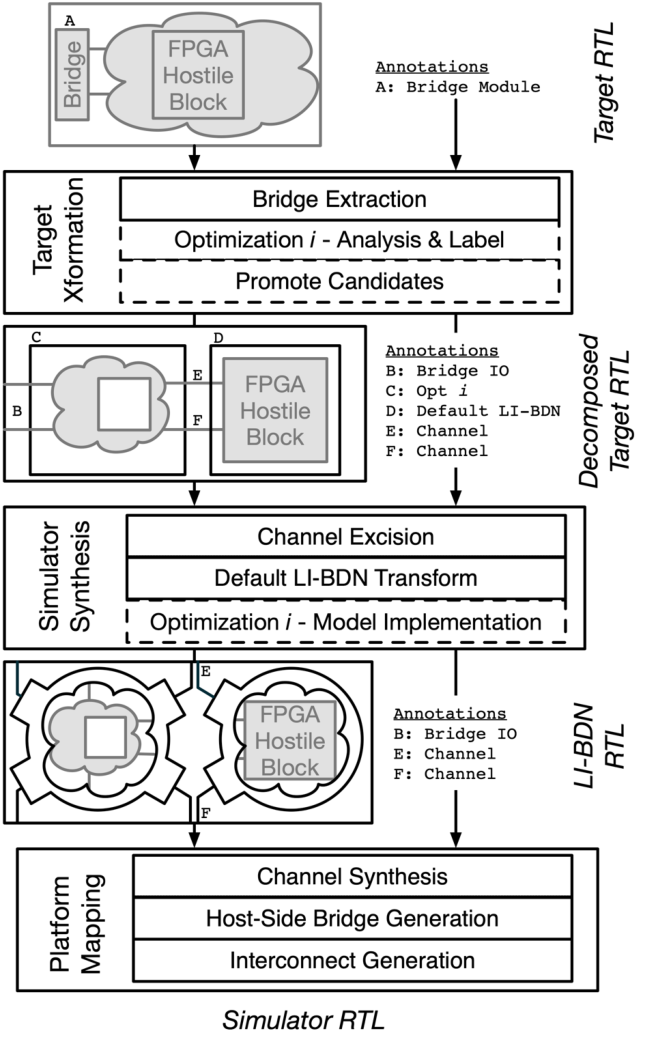
\includegraphics[width=0.8\textwidth]{figures/gg-toolchain.pdf}
    \caption{Core phases of the Golden Gate compiler and a high-level depiction of the transformations made to the underlying target.}
    \label{fig:gg-toolchain}
\end{figure}

\begin{enumerate}

\item \textbf{Target Transformations}: The frontend of the compiler. Here the
module hierachy is mutated in preperation for host decoupling. Bridges are
extracted, unsynthesizable debugging constructs are replaced and bound to a
bridge interface. Primitives identified for optimization are wrapped in a
module and labelled. Top-level instances correspond one-to-one to units in the
eventual simulator, and top-level connectivity define edges in the graph.

\item \textbf{Simulator Synthesis}: Here, top-level modules are transformed
into, or replaced with equivalent units. The output circuit consists of a
series of unconnected unit instances. Connectivity between units is captured in
channel annotations between top-level IO.

\item \textbf{Platform Mapping}: This consists of the Simulation Mapping and
Platform Mapping passes of MIDAS. A chisel-generated wrapper instantiates all
channel implementations and invokes bridge generators. The resulting output
circuit is compatible with the same FPGA projects as MIDAS-generated
simulators, and plugs into FireSim's existing flow.
\end{enumerate}

\subsection{Annotations}
Golden Gate relies on FIRRTL's annotation system to communicate information about the
circuit from transform-to-transform instead of an auxiliary
datastruture that persists across transformations. The main motivation for doing so was to make transforms in the
compiler robust against running lowering or optimization transformations
between them, as the FIRRTL compiler framework provides callbacks for defining
how annotations should be modified when the circuit structures they target are
changed (a process known as \emph{renaming}). We describe the key annotations here:

\begin{itemize}
\item \textbf{Bridge Annotations} label instances in the target for which a custom unit will be generated.
    In addition to providing a target module, they carry a fully qualified class name
    of the Bridge Module to be generated and it's optional constructor parameter. Finally,
    annotation enumerates the names of all of it's channel annotations.

\item \textbf{Connection Annotations} label connections between modules that correspond to units and bridges of the simulator, and
    carry the information required to generate a channel them. This consists of
    a list of sources~(\texttt{sources}), IO fields on the instance that drives the connection
    (and thus sources the the tokens), and sinks~(texttt{sinks}), IO fields on a module
    receiving those connections. Channels carry additional non-target metadata,
    including a globally unique string identifier~(\texttt{globalName}), as well as a case class~(\texttt{chInfo}) that
    captures target properties of connection and channel-implementation hints.
    The \texttt{chInfo} has subtypes to indicate whether the channel is latency
    insensitive and and should be implemented with a queue-type channel, or is a pipe-type channel.

\item \textbf{Port Annotations} label groups of IOs in a module as corresponding to a source or a sink of a
    channel. A list of sources or sinks in connection annotations (which point
    at instances of the module) must agree with the port annotation on the
    module itself. Port annotations are primarly consumed by transformation passes and provide the simplest means
    to look up how the I/Os of the module should be divided into channels.

\item \textbf{Model Annotations} serve a similar function to BridgeAnnotations, in that they label a
    module as being a unit. Unlike bridges however, instances of the target module
    are not extracted from the design hierarchy, but instead are promoted to
    the top-most level of the design hierarchy, so that they can later be
    transformed by the compiler in Simulator Synthesis.
\end{itemize}

At the start of compilation, bridge annotations are present, with connection
annotations labelling their interfaces.  Model annotations may also present
alongside specific optimization annotations.

\section{A Walkthrough Compilation - Target Transformation}
The transform order for Golden Gate is statically defined in
\texttt{MidasTransforms}\footnote{https://github.com/firesim/firesim/blob/1.8.0/sim/midas/src/main/scala/midas/passes/MidasTransforms.scala},
. Target transformation consists of all transformations before
\texttt{ChannelExcision}.

The primary function of target transformation is to coerce the design's module
hierarchy into a form that matches the eventual simulator topology: top-level
instances map to unit instances~(nodes) and top-level connections map to
channels~(edges).

Target transformation begins with an initial lowering and optimization, and
checks the validity of the input circuit for GG complication (namely, circuit
presents no top-level IO \texttt{EnsureNoTargetIO}). Next, Golden Gate
runs assertion and printf synthesis. Under-the-hood do not fundamentally differ
from what was described in our DESSERT publication~\cite{DESSERT}, with the
exception the generated top-level IO drive a bridge~(more on this later).

Bridge Extraction~(\texttt{BridgeExtraction}) runs, finding all modules
annotated with a BridgeAnnotation and removes them. Connections to instances of
the bridge are replaced connections to their instances with connections to new
top-level IO. A single bridge module, with multiple instances will produce N
sets of ports at the top-level. The bridge and connection annotations are
"promoted" to point at these new top-level interfaces. Bridge annotations are
replaced with a form of annotation that targets top-level IO
(\texttt{BridgeIOAnnotation}, instead of a module, but is otherwise indentical.
Connection annotations are assigned new \texttt{globalNames}, to ensure they
are unique, with their corresponding BridgeIOAnnotations updated to reflect
that.

Next, Golden Gate prepares to preform it's hierarchy manipulations by adding a
wrapper module around the existing design~(WrapTop). The previous
top-level module will become a unit in the simulator.

Then Golden Gate finds all modules labeled with a model annotation, and
promotes their instances to the fame wrapper. This process is nearly identical
to bridge extraction, but the module is not completely removed. Just as in
bridge extraction, one annotated model will produce as many top-level instances
as there were instances of the module in the design hierarchy.  At this point
the connectivity within the wrapper reflects the star-topology of the eventual
simulator: the original source module is the hub, all promoted modules and
bridge interfaces connect to it.

With the module hierarchy manipulations done, Golden Gate completes target
transformation by fleshing out missing
annotations~(\texttt{FAMEDefaults}). This primarily consists of labelling
all inter-model connectivity with connection annotations. This pass makes no
attempt to group connections into a single channel: every ground type
connection gets a single annotation and thus will get independent channel
implementations.

\section{Simulator Synthesis}

Simulator synthesis is so named, because it begins introducing host-time constructs in to the circuit,
most notably with the execution of the default FAME transformation.

Simulator synthesis begins, by removing all inter-model connectivity and
replacing it with top-level IO~(\texttt{ChannelExcision}). Connection
annotations are promoted to point at these new interfaces. Only now are port
annotations added~(\texttt{InferModelPorts}), since connections between bridges
and models are uniform (they are all connections to top-level IO).  This
transformation ensures that connection annotations on instances of the same
module agree how ports correspond to channels. Since \texttt{FAMEDefaults}
makes no attempt to group channels currently, this mainly serves as a
consistency check on bridge-bound channels and ensures no connection
annotations have been lost.


The bulk of the complexity in simulator synthesis is contained in it's default
FAME transform (\texttt{FAMETransform}. It has two fundamental tasks: First, it
transforms all top-level models, including those that will be optimized later,
into units using a default, wrapper-based LI-BDN transform~(described
previously and shown in Figure~\ref{fig:libdn-wrapper}). The transform groups
ports into decoupled interfaces by consume the port annotations for the model
in question. References to ports are replaced with references to the payloads
of these channel ports. Valid and ready signals are used to to build out the
control circuitry circuit shown in Figure~\ref{fig:libdn-wrapper}, however,
this logic is appended to the existing module (to avoid introducing another
level into the module hierarchy). Finally, all references to the target clock
are replaced with a reference to the output of the clock buffer.  The clock
buffer itself is left as a black-box that will be implemented later for the
desired host FPGA.  Second it replaces the IO and connectivity in the fame wrapper with decoupled equivalents. For
example, a boolean driven by a model is replaced with a three bit interface:
valid and the boolean payload is driven by the model, and ready (backpressure)
is driven by the interface in the FAME wrapper. Connection annotations are
updated to point at the payloads of these channels.

Here, optimization transformations can be inserted to replace the default
implementations with optimized ones.  At this point the design is nearly ready
to be linked against the simulation wrapper.  Transforms add a default clock
buffer implementation (\texttt{DefineAbstractClockGate}), and wire up the
host-clock and reset to all units in the circuit(\texttt{ConnectHostClock}).

\section{Platform Mapping}\label{sec:gg-platform-mapping}

In Golden Gate, platform mapping is responsible for both implementing all
channels (previously simulation mapping in MIDAS), in addition to elaborating
all remaining simulation collateral, such as bridges, and resource interconnect
(previously, platform mapping in MIDAS). This happens in single Chisel
invocation.

\subsection{Channel Synthesis}
Elaboration of this module is driven by the user-defined parameter's instance,
which as in MIDAS specifies properties about the host-platform, and by
annotations in the now transformed target.  Channels are generated in a wrapper
circuit~(\texttt{SimWrapper}) that directly links against the transformed RTL.
This wrapper circuit processes connection annotations, generating a channel
implementation for each, generating a channel implementation for each.  There
are three cases, connection annotations that posses both sources and sinks
tconnect two models in the transformed RTL. These are \emph{loopback} channels
that drive and input and output interface on the transformed target. Conversly,
annotations that have either an empty sources or empty sinks paramaters connect
are sunk and driven by as bridge module, respectively. If a channel is sunk or
driven by a bridge, the channel implementation has it's dequeue or enqueue side
interface exposed to the next level of the design hierarchy.

In all cases, the type of channel generated is parameterized by the
\texttt{channelInfo} field of the annotation. The decoupled channels, as in
MIDAS, always instantiate a model of a fully decoupled, 2-deep queue. Pipe
channels have a configurable latency. Default bridge implementations always
emit channel annotations with latency = 1 to improve FMR, and to maintain the
performance characterisitics of legacy MIDAS simulators. When no additional
models are extracted (i.e., the simulator consists only of the hub unit and
bridges) the expected FMR is identical to MIDAS.

When additional models are extracted, they are always directly wired to one
another, since the compiler currently cannot find and extract registers between
two models~(\texttt{FAMEDefaults} labels these channels as wire-type). This has
the effect of making all multi-model simulators, using the default FAME
transform, execute with an FMR of at least two\footnote{It is possible to build
simulators with unity FMR, if an optimized model's outputs can runahead. A time
of writing, we have no such implementations.}

\subsection{Bridge Instantiation}
The next-level of the module hierarchy corresponds directly to the wrapper
circuit generated in MIDAS's platform mapping. Instead of using an endpoint
map, Golden Gate iterates through each bridge annotation, and reflexively looks
invokes the a constructor for the requested BridgeModule. I/O between the elaborated
bridge instance and the simulation wrapper are connected by looking up the
corresponding channels via their \texttt{globalName}s.

Resource-interconnect generation is identical to MIDAS's, and for the same
input design, the emitted header is the same. All MIDAS endpoints were ported
to use the new Bridge system, without changing the host-software.

\section{ICCAD 2019 Case Study: Multiported BRAMs}

Armed with the machinery to selectively extract and reimplement FPGA-hostile
componenets of the target design, in our ICCAD2019 we set about optimizing
multi-ported RAMs~(we previously introduced this example in
Section~\ref{sec:iron-law}).  ASIC multi-ported RAMs are a classic culprit of
poor resource utilization in FPGA prototypes, as they cannot be trivially
implemented in BRAM and are instead decomposed into LUTs and
registers~\cite{FPGAGap2}.  While using double-pumping, BRAM duplication, or
FPGA-optimized microarchitectures~\cite{MultiportXOR} can help, here we use Golden Gate to
automatically substitute a decoupled model to further reduce resource
utilization. This enables a target memory with $M$ asynchronous read ports and
$N$ write ports to be implemented by time-multiplexing by time-multiplexing
a single dual-ported BRAM. In contrast to the static time-multiplexing described
in \cite{APortNetworks} and \cite{fabscalarfpga}, our optimization can decouple arbitrary target
memories and replace them with an optimized model (described in more detail in
Section~\ref{sec:case-study:model-uarch}) without any constraints on the structure or timing of the
target design.

\subsection{Our Target ASIC}

We evaluated this optimization on  multi-core SoC instances produced by the Rocket Chip
Generator~(\cite{rocketchip}, described in
Section~\ref{sec:ucb-bar-recent-work}). Specifically, we studied two different
``core complexes''---consisting of the cores and inner caches---each based on a different RISC-V core
implementation: Rocket~\cite{rocketchip}, an in-order scalar core, and
BOOM~\cite{BOOM}, a unified physical register file, superscalar out-of-order core.
In each case, we evaluated the impact of substituting each core's floating
point~(FP) and integer register files for an optimized memory model.  Since
these cores can be generated with many different register files
configurations, we describe register file parameters for the instances we studied
in Table~\ref{tbl:regfile-specs}.

\begin{table}[h!]
\centering
\begin{tabular}{c c c c c}
\hline
\multirow{2}{*}{Type} & \multirow{2}{*}{Size} & Read & Write & BMC \\
 & & Ports & Ports & Runtime \\
\hline
Rocket integer & $31 \times 64$b & 2 comb. & 1 & $445\,\text{s}$ \\
Rocket FP & $32 \times 64$b & 3 comb. & 2 & $334\,\text{s}$ \\
BOOM integer & $100 \times 64$b & 6 comb. & 3 & $637\,\text{s}$ \\
BOOM FP & $64 \times 64$b & 3 comb. & 2 & $372\,\text{s}$ \\
\hline
\end{tabular}
    \caption{Register file specifications for the two target cores.}
    %Each is replaced with an optimized model; resource utilization and simulation speed is compared with the baseline FPGA mapping.}
\label{tbl:regfile-specs}
\end{table}

\vspace*{-5mm}
\subsection{Model Microarchitecture}
\label{sec:case-study:model-uarch}
The optimized memory model is structured around a dual-port, synchronous read memory that stores the
contents of the simulated memory, which, unlike the FPGA-hostile memory it models, can be implemented in BRAM.
Access to this memory
is mediated by an arbiter that selects a maximum of two target read/write requests per host clock
cycle; this arbitration is dynamic, based upon when the tokens associated with individual ports
arrive on their associated decoupled interfaces. As shown in Figure~\ref{fig:model-uarch},
an FSM is associated with each target port; together, this vector of FSMs tracks the
model's progress in consuming input tokens, performing BRAM accesses, and producing output tokens.

%\subsection{Verifying the Model With LIME}
%
%The \LIME flow can be applied to any Golden Gate simulation model, but it is especially useful for the widely applicable memory optimization.
%While each instance of the model is the output of a parameterized generator,
%checking a large subspace of the optimized models using \LIME
%provides a high degree of confidence in the correctness of the transformation. In multi-core SoC, checks are
%also amortized across multiple identically parameterized memories.
%
%From a usability perspective, \LIME is an extremely convenient tool to find bugs in optimized
%simulation models of highly ported memories.
%Implementation bugs may appear only in specific corner cases, such as a certain interleaving of
%I/O token arrivals interacting pathologically with the write collision semantics of the
%memory. In contrast with labor-intensive, model-specific directed random
%testing, \LIME offers a push-button bounded model check that finds all bugs that can manifest within
%the time horizon of the bound. While a 20-cycle BMC bound has sufficient depth to cover the full
%space of I/O token arrival interleavings over several target cycles,
%Table~\ref{tbl:regfile-specs} shows that this bound results in quick runtimes; longer BMC checks can
%be amortized over many uses of common configurations.
%\vspace*{-0.3in}
%\begin{figure}[h!]
%  \centering
%  \includegraphics[width=.7\columnwidth]{figures/async-mem-model-microarchitecture.pdf}
%  % graffle2pdf -c all midas-graphics/graffle/async-mem-model-microarchitecture.graffle figures/async-mem-model-microarchitecture.pdf
%  \vspace{-0.22in}
%  \caption{A microarchitectural sketch of a three-read, two-write, optimized Golden Gate memory model.}
%  \label{fig:model-uarch}
%\end{figure}
%\vspace*{-5mm}
%\begin{table}[h!]
%\centering
%    \vspace*{-2mm}
%    \begin{tabular}{c c c c c c}
%    %\begin{tabular}{S[table-format=3.0] S[table-format=3.0] S[table-format=3.0] S[table-format=3.0] S[table-format=3.0]}
%    \hline
%        & R4 & R16 & B4 & B5 & B6 \\
%    \hline
%        Baseline  & 135 MHz & 60 MHz & 90 MHz & N/A    & N/A \\
%        Optimized & 135 MHz & 60 MHz & 80 MHz & 60 MHz & 50 MHz \\
%        %Rocket 4 core & 135   & 135  & 135     & 6.4 \\
%        %Boom 4 core   & 90    & 2.1  & 80      & 9.1 \\
%        %Boom 5 core   & N/A   & N/A  & 60      & 9.3 \\
%        %Boom 6 core   & N/A   & N/A  & IPR     & 9.1* \\
%    \hline
%\end{tabular}
%    \caption{$f_{FPGA}$ for successfully implemented simulators.}
%    \vspace*{-0.25in}
%\label{tbl:simulator-speed}
%\end{table}
%\vspace*{-0.2in}

\subsection{Adding the Optimization To Golden Gate}

To enable our optimization in Golden Gate, we added an analysis pass that finds annotated
RAMs and a model-implementation pass that inspects the
parameters of the target RAM~(ports, width, and depth) and invokes our
model generator~(Section~\ref{sec:case-study:model-uarch}). We also annotated the register file RAMs in the target RTL.
With these passes enabled, Golden Gate detects and promotes a pair of candidate RAMs for
each core of the SoC during target transformation. In simulator synthesis, the implementation pass consumes the RAM modules
and produces equivalent models. At this point, the rest of the flow proceeds as described
in~Section~\ref{sec:gg-platform-mapping}).
Enabling memory substitution adds 5 and 69 seconds of FIRRTL compile time to the quad-core Rocket
and hexa-core BOOM configurations, respectively the smallest and largest designs we studied. This is negligible
relative to their FPGA compile times of 6 and 22 hours.

\subsection{Results}
The results of applying the multi-ported memory optimization are shown in
Figure~\ref{fig:iccad19-utilization}. Optimized BOOM designs use 26\% fewer LUTs than baseline designs, 
allowing two extra cores~(B5, B6) to fit on a single VU9P.
The sixteen-core, Rocket-based design also saw an 7.8\% reduction in LUT utilization over the baseline, despite
having lesser-ported, shallower regfiles. We report FPGA frequencies for all designs that closed timing
in Table~\ref{tbl:simulator-speed}.

As discussed in Section~\ref{sec:iron-law}, replacing components of the target with
decoupled models will impact the FMR, therefore lowering simulation throughput. 
FireSim, being a decoupled simulator, generally has FMR greater than unity. In
particular, FireSim uses a last-level-cache and DRAM model~\cite{fased} (utilization included in \emph{FireSim Misc.} of Figure~\ref{fig:utilization}) to
inmplement deterministic simulation of the target's outer memory system using host FPGA DRAM.
When booting a Buildroot Linux distribution, adding multi-cycle RAM models increases FMR
from 1.9 and 1.8 to approximately 6.9 and 9.3 for Rocket and BOOM designs, respectively.
FMR is a function of the highest port-count model in each target,
but is nearly constant across core count, since the models are not
combinationally coupled and therefore execute concurrently.
Finally, we note that the performance penalty of using multi-cycle models may
often be less than that of partitioning---while
using only one FPGA.

\begin{figure*}[ht]
\centering
    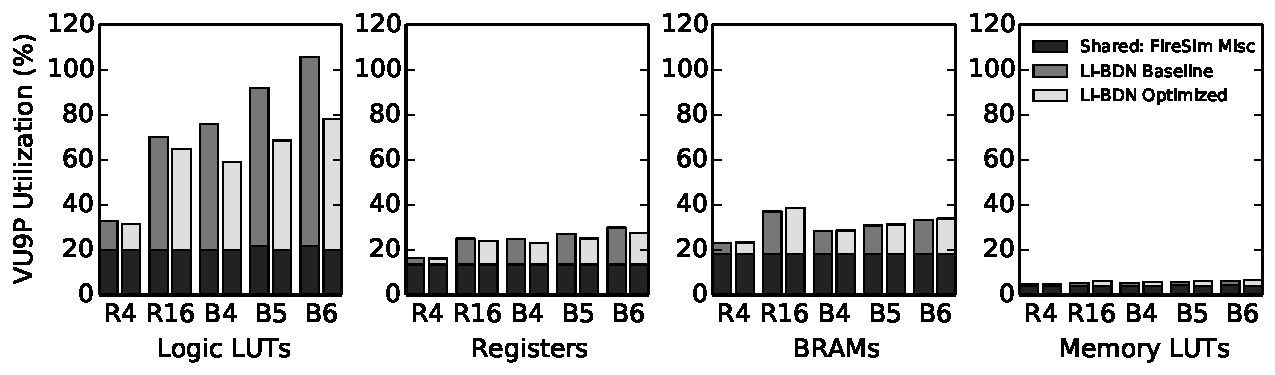
\includegraphics[width=\textwidth]{figures/resource-utilization-vu9p.pdf}
    \vspace{-0.30in}
    \caption{Total VU9P resource utilization for baseline and optimized simulators. Designs are labeled R[ocket]$N$ or B[oom]$N$, with $N$
    corresponding to core count. \emph{FireSim Misc} accounts for all resources in
    the Amazon-provided shell (v1.4.0) and FireSim hardware for co-simulation; this is fixed across all designs.  We omit DSP48s and URAMs as they are constant across all designs and lightly used. \emph{Baseline} penta- and
    hexa-core BOOM designs failed in placement due to over-utilization--
    we report post-synthesis utilization. \emph{Optimized} versions of the same designs use 26\% fewer logic LUTs, and successfully place and route.}
    \label{fig:iccad19-utilization}
\end{figure*}

\section{LIME: Verifying Optimizations}

\section{Bridges In More Detail}
%
%\subsection{Autocounter}
%
%\subsection{Synthesized Assertions}
%
%\subsection{Synthesized Printfs}
%
%Simulator QoR?
%
